% 1961 年全国卷第 8 题：圆环铁皮的五分之一扇形。
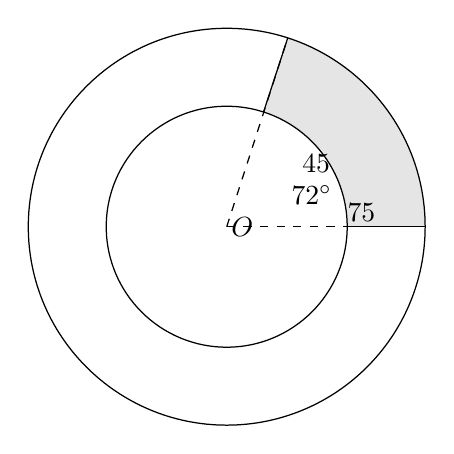
\begin{tikzpicture}[scale=0.9, line width=0.45pt,
  every node/.style={inner sep=1.5pt}]
  \coordinate (O) at (0,0);
  \fill[gray!20] (2.8,0) arc (0:72:2.8)
    -- (0.52,1.62) arc (72:0:1.7) -- cycle;
  \draw (O) circle (2.8);
  \draw (O) circle (1.7);
  \draw (2.8,0)--(1.7,0);
  \draw (0.86,2.66)--(0.52,1.62);
  \draw[dashed] (O)--(2.8,0);
  \draw[dashed] (O)--(0.86,2.66);
  \node[anchor=west] at (O) {$O$};
  \node[anchor=south] at (1.9,0) {$75$};
  \node[anchor=south west] at (1.0,0.7) {$45$};
  \node at (1.2,0.45) {$72^\circ$};
\end{tikzpicture}
